
%(BEGIN_QUESTION)
% Copyright 2009, Tony R. Kuphaldt, released under the Creative Commons Attribution License (v 1.0)
% This means you may do almost anything with this work of mine, so long as you give me proper credit

Suppose the wire between terminal number 7 and input channel IN5 breaks open in this PLC-controlled motor starter system:

$$\includegraphics[width=15.5cm]{i02378x01.eps}$$

Determine the effect this fault will have on the system, and identify how that fault could be diagnosed using the color-highlighted RLL program display in the editing software of a personal computer connected to this PLC.

\vfil

\underbar{file i02378}
\eject
%(END_QUESTION)





%(BEGIN_ANSWER)

This is a graded question -- no answers or hints given!

%(END_ANSWER)





%(BEGIN_NOTES)

Before we are able to analyze the effects of this wiring fault, we need to determine how the system is {\it supposed} to function.  Being that both the Start and Stop pushbuttons are wired normally-open (NO), the PLC must be programmed to expect an activated input when the corresponding button is pressed.  That is to say, an energized Start input (channel 3) tells the PLC to start the motor, while an energized Stop input (channel 5) tells the PLC to stop the motor.

\vskip 10pt

If the wiring from the Stop pushbutton fails open, channel 5 will always be de-energized, and therefore the PLC will ``think'' the Stop pushbutton is never pressed.  The consequence of this fault is that the operator will not be able to stop the motor.  This fault will be evident when the ``Stop'' button is pressed and the coloring of the virtual contact associated with input channel IN5 remains unchanged.

This fault will also be evident by noting that the status LED on input IN5 never lights up when the ``Stop'' pushbutton is pressed!

%INDEX% PLC, troubleshooting: determining response of specified system fault(s)

%(END_NOTES)


